\section{Evaluation}
\subsection{Project Achievements}
All four primary objectives of this project have been implemented, and as such the project is considered a success. The four primary objectives of rendering sheet music, extracting data from the sheet music files provided, processing queries on the data collected and expanding the collection using online sources were set as each contribute a way to automatically organise, expand and view their collection and are achievable, measurable objectives. The sub sections below go into each objective in detail, in order to convey any particular technical challenges which had to be overcome to reach each objective.
\subsubsection{Rendering System}
This project implements the ability to view sheet music stored as MusicXML files. Composition software such as Finale by \cite{finale}, MuseScore by \cite{MuseTour}, and Sibelius by \cite{avid} each implement their own file format and provide export and import options to and from MusicXML. Focussing on their own file format means that the input and output of MusicXML is less precise, proven by the number of issues in the MuseScore issue tracker shown in figure \ref{fig:issues}.

\begin{figure}[H]
\centering
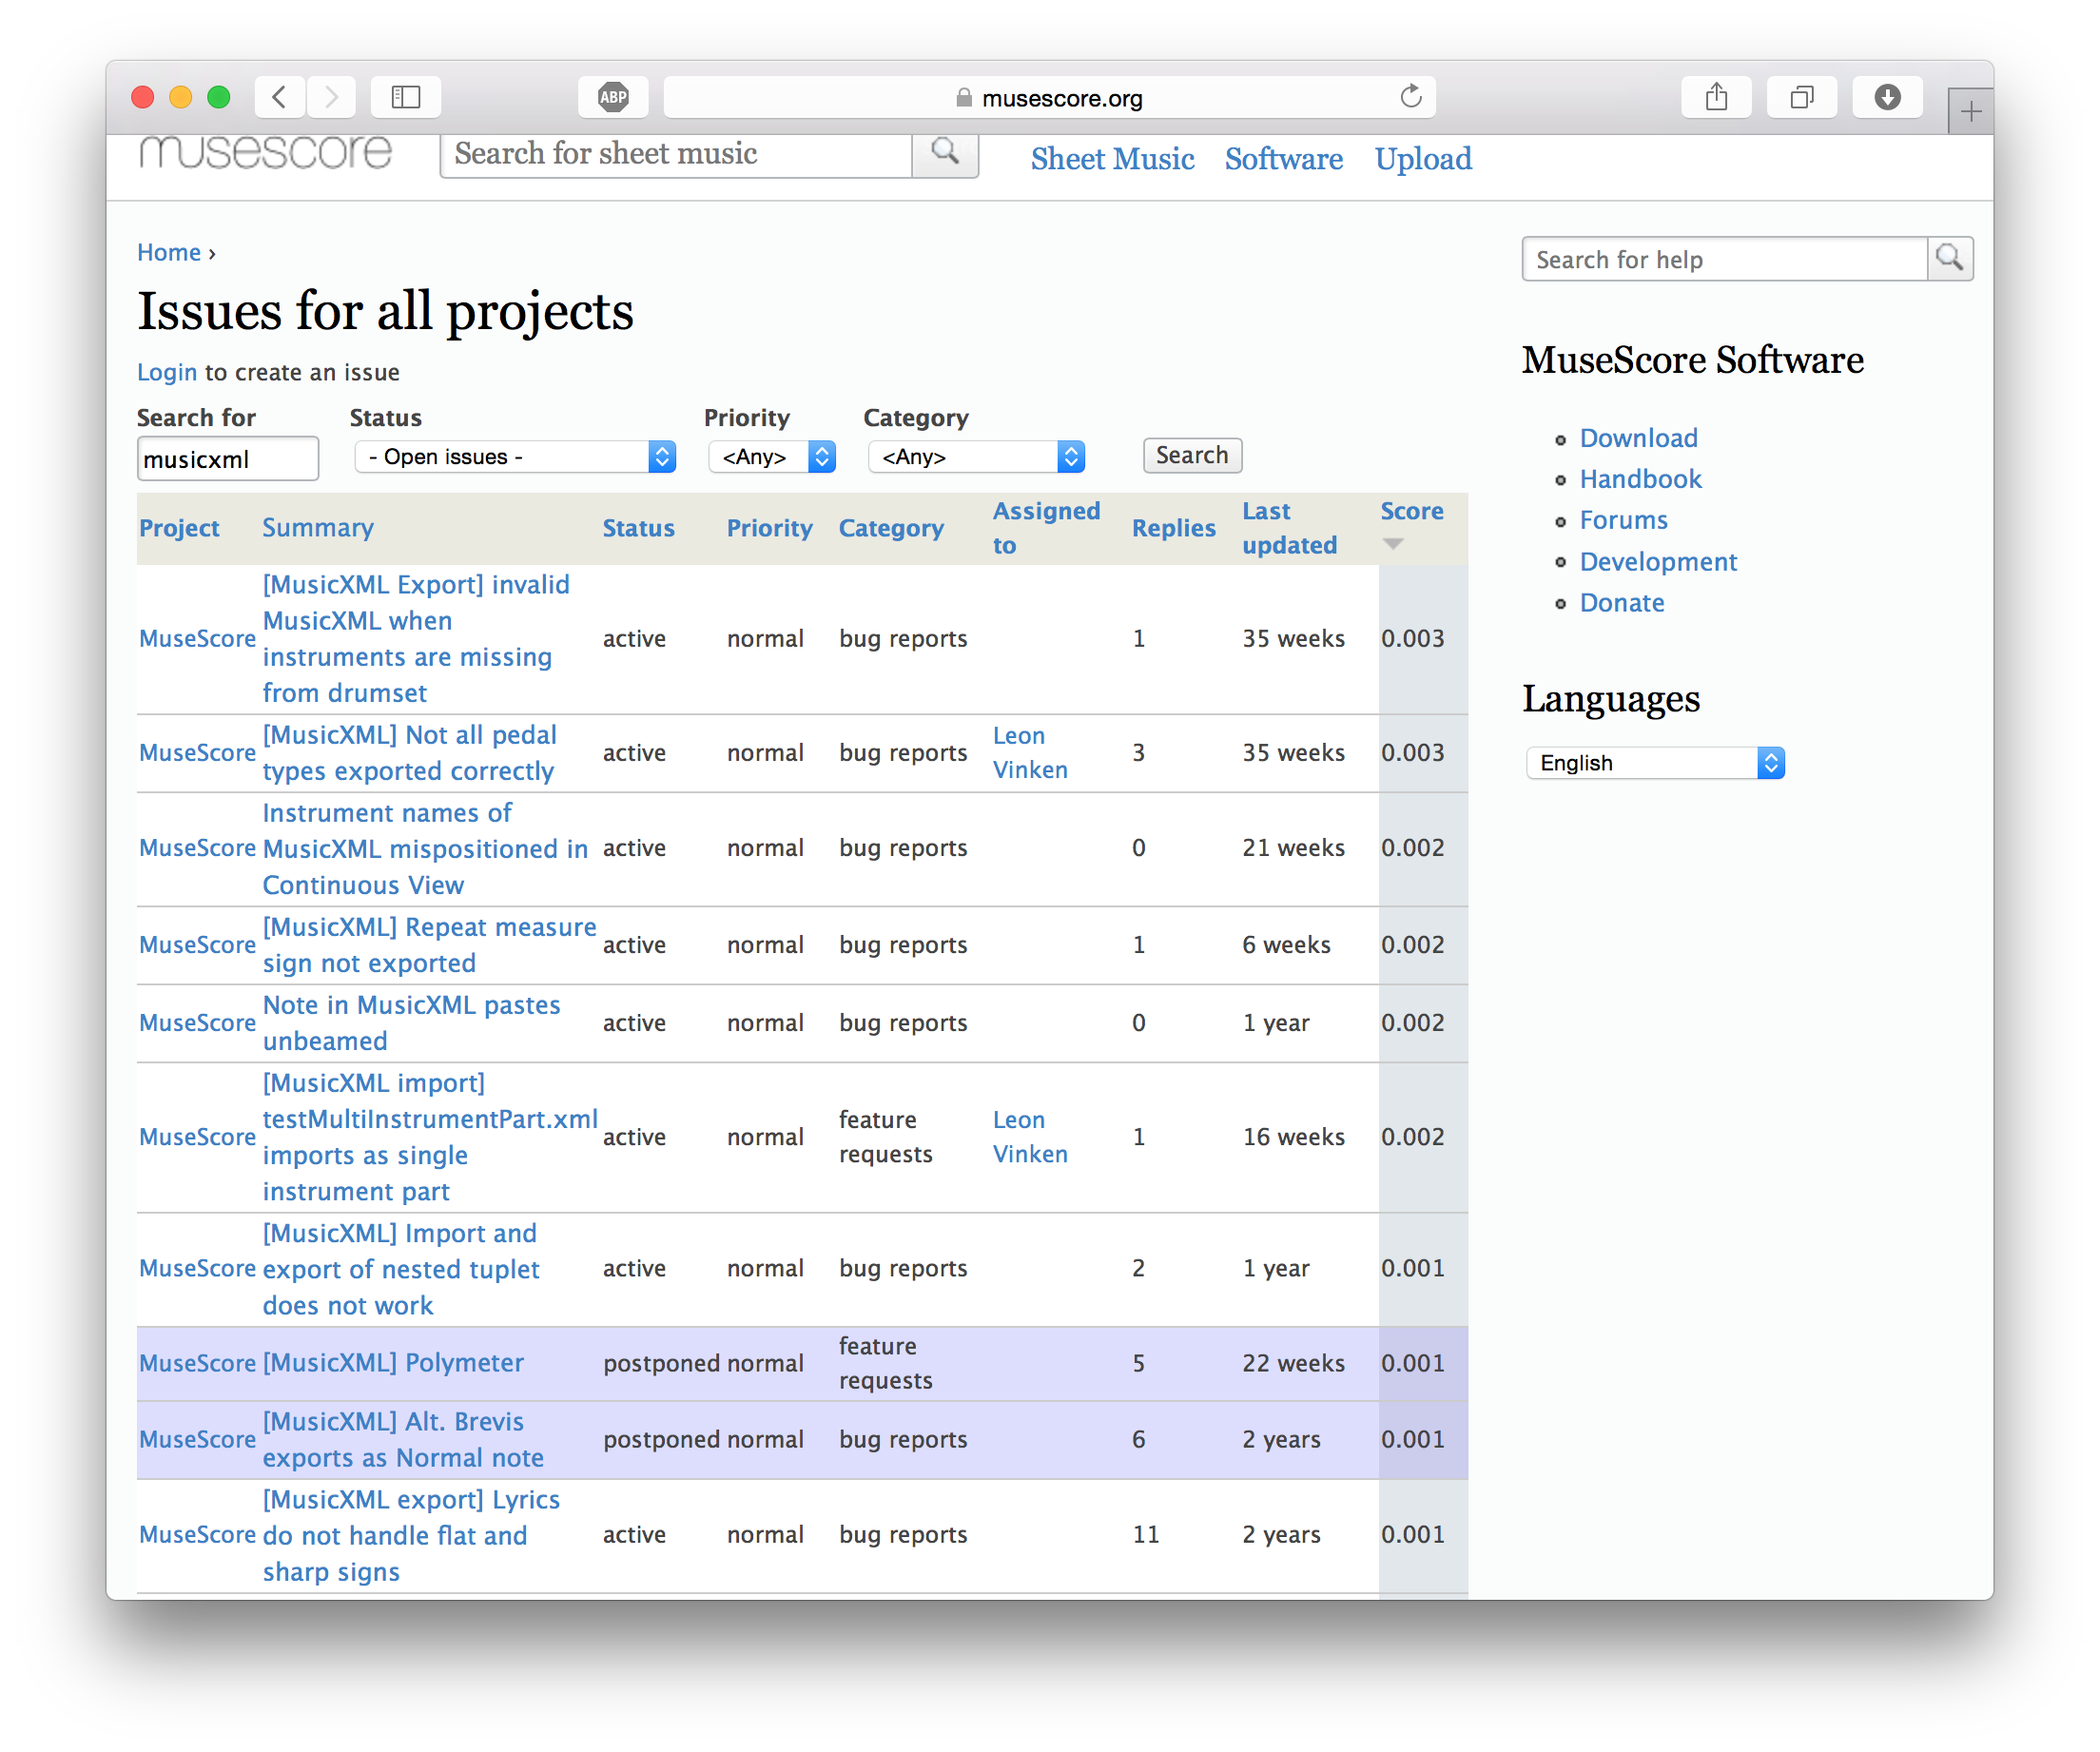
\includegraphics[width=400pt]{issue_tracker}
\caption{Issue tracker for the MuseScore project}
\label{fig:issues}	
\end{figure}

This project focussed on MusicXML, and therefore the input and output of elements should be more precise than the software referenced in the previous paragraph. This is achieved with low coupling to either format, as the system implements an object structure to manage communications of data into or out of the system.

Technical challenge was overcome in designing the objects used in the system around two separate input and output formats which had very different design aims for how sheet music should be stored and processed. This was achieved in the late stages of development through redesign with the test harness confirming that implementation of the redesign did not introduce any problems.

The classes and scripts for input and output are loosely coupling to other features, meaning that it would be possible for a new developer or new project to take this code and use it in a different context without requiring other objectives and features to make the system work. Using the SAX method of XML parsing means that the renderer can easily be extended and iteratively improved to handle more and more complex XML information.

\subsubsection{Metadata scanning}
This project implements the ability to organise sheet music through the extraction of information about each piece of sheet music. The information is general in the sense that the data collected is of relevance to the majority of pieces of music and all instruments. 

Further to automated scanning, the system allows users to create their own playlists. The search with suggestions system described in section 5.1.3 is modular, so the playlist creator has the same query structure and abilities as the general search function.

The metadata model created for this project was designed so that it would be of the most use to all performers. This design decision was made so that the application would be useful to a cross section of musicians, and with the additional intent of defining a standard model for future projects to implement.

\subsubsection{Search and Playlist operation}
From the extracted metadata it is be possible to search the catalog of music for specific requirements, such as key, clef, meter, time signature. This is achieved using a string of user input which is transformed into queries, which are handled by the data layer.

Suggestions for what the user might be looking for are updated in near-real time and avoid blocking the user from updating their query using multi processing. The challenge overcome here was designing the syntax for a non-technical user, but providing enough scope for complexity to produce a wide range of queries, and was achieved using a mix of language processing and new query syntax.

The system also uses the meta information to produce auto generated playlists which are listed in the user interface. Playlists provide an alternative viewing format to queries, in that it provides a list of pieces which are related to each other, and was made part of the search objective as this is a way in which the data can be used to create an organised user interface. 


\subsubsection{Importing Online APIs}
The application makes it possible to connect to online music collections and search them using the same user interface as searching for local files.

A general API class was implemented in this project to handle communications with networked sheet music collections. This class will be useful to future applications or extensions as new sheet music collections can easily wrap their own APIs in this class, and implement them without needing too many requests or changes at code level.

Whilst the API initially downloads an XML file in order to extract information for every piece in the source, when a user decides to download a file, the API will request PDF files where available. This means that the renderer does not have to be used, which reduces the processing overhead needed for downloaded files to be displayed.

Furthermore, applying the same model and metadata scanner used on local files to online files makes this feature more useful, as users can search their local collections and online collections using the same queries. This enables users to expand their collections without leaving the application or changing their behaviour.

\subsubsection{Cross Platform Capabilities}
All four of the objectives and the graphical user interface for this project are built to be used on the three most popular operating systems - Mac OSX, Windows 8.1, and Ubuntu (GNU/Linux).

A packaged version of this application has been produced for OSX, with work to produce a Windows installer program ongoing. This was achieved by paying close attention to which libraries were available in Python and avoiding any which did not explicitly state they would function cross platform.

\subsubsection{Graphical User Interface}
All of the objectives and functions of the program are accessed from the same user interface, which provides several views and options to the user depending on how they wish to view and organise their music. As well as automatic organisation, this also provides a create playlist function which allows users to create sub-collections of music which are related to each other, or create set lists for orchestras. The user interface is shown in figure \ref{fig:annotated}, and also in the user guide in the appendix.


\subsection{Further Work}
\subsubsection{Improved Rendering Capabilities}
The current renderer has the capability to handle much of the most common symbols used in sheet music. This varies from the notes themselves to dynamics and articulation, and includes all of the symbols mentioned in the problem context. The rendering system covers all instruments which have parts written using the standard Western Classical sheet music notation, such as Clarinet, Cello, Piano, and Trumpet.

However, this objective in particular took more time than originally intended or expected, and despite the importance of a working renderer in order for a musician to view their sheet music, it was decided that covering the majority of use cases was enough. As such, some specific areas of notation including guitar tablature, drum tablature, lyrics and some notation used in foreign countries and previous generations of western music were ignored. This was due to it becoming obvious that some of these areas would take too much time modifying the current structure, and others were not considered to be important enough to take precedence over the other objectives.

The decision was therefore taken to limit the functionality of the renderer at the advantage of having more time to work on the remaining objectives, but with clear instruction noted for future development on which areas needed to be improved or included in the future. This was achieved using the test cases released by \cite{Lilypond}, with visual checking of the output and reporting issues on which test cases failed, and why they were considered failures. It is important to note that the developer ensured that all of these test cases did not cause a program crash, and that all test cases generated some form of PDF output.

\subsubsection{Creation and release of an Open Rendering Library}
This project had baseline requirement of developing a sheet music rendering system in order to achieve the "view sheet music" part of the aim.  The baseline requirement was needed because there was no third party library available for download and installation which would do the same job without extracting the code from a previous project \parencite{pypi}.

It is the intention of the developer to take the current rendering system and produce an independent rendering library, which will be used by the project but also released into the Python Package Index (PyPi), making it available to be downloaded and used by anyone else who needs to use a rendering system.

\subsubsection{Secondary Objectives}
The three secondary objectives were not included in the final project outcome.  The decision was taken to ensure that the three primary objectives were all tested thoroughly, and that the application is a rounded and polished product, with packaging for OSX and Windows taking precedence over features which may or may not be finished to the same quality as the four primary objectives. 

The first secondary objective, Sound output, was not implemented because the developer felt that it would take time researching the best file format to use for sound output. Furthermore, the developer would need to research and learn to use the libraries needed in python to produce those files using music symbols. Lilypond supports output to midi using the $\midi{}$ command, but this would tightly couple the sound output objective with the rendering objective. This area was researched however in the sense that the developer planned the structure for producing sound output, which would be the same implementation as the rendering objective, using a method call like ToMidi() or ToMp3.

The second secondary objective, image input, was not implemented because the developer felt the area high risk because of the potential amount of work and research required. Research was put into finding third party OMR libraries like \cite{audiveris} and \cite{openomr}, but Audiveris did not appear to have an OSX installer which is the developer's development platform. OpenOMR did not have sufficient documentation for the developer to be able to learn the functionality in time, and both projects are written in Java which means that the project would need to implement some sort of extension to communicate between the platforms.

The third secondary objective, difficulty rating, was not implemented because the developer did not have sufficient time or knowledge of machine learning algorithms. Whilst the developer had a clearer picture of how to implement this objective, using contextual analysis of each symbol against a knowledge database, the developer felt the aspects to be researched had the potential to take too much time understanding how they worked. Research here was done into collecting data about which instruments had difficulty with particular aspects of music, which involved producing a survey which was then given to a wide range of non-technical music. The results of this survey are given in the appendix, and will be used in development of this objective in the future.

The developer will prioritise the second objective, image input, because it is believed that this would be of the most use. Implementation of image input would make the process of importing and organising new music from physical copies completely automatic if the application implemented links to scanners and cameras, which would reduce the time and effort taken to digitise sheet music collections.

\subsubsection{Porting to Linux based operating systems}
The intention of the developer was to create a packaged version of the application for the three major operating systems - Windows, OSX, and Ubuntu. 

Time constraints meant that the developer had to prioritise based on usefulness and user count for the chosen demographic, and it was predicted that Windows and Mac OSX would be the most used operating systems by musicians.

Whilst it is expected that the GNU/Linux installer will be relatively simple to create, the developer chose to leave this process to after the demonstration.

\subsection{Future Developments}
\subsubsection{Porting to Raspbian}
It is hoped that a Raspberry Pi compatible version can be created which may involve optimising certain features in order to fit on a smaller operating system. 

With this comes potential for new input mechanisms, such as the PiPiano, an add on board which allows users to input music using buttons arranged in a piano keyboard organisation \parencite{pipiano}, and new output mechanisms, such as Sonic Pi, which was created as an educational tool to teach children how to program using music as the inspiration and final output \parencite{sonicpi}. 

\subsubsection{Symbolic Searching}
The current project uses text input formatted in a particular manner in order to query the database. It is hoped that in future, a Music Ngram searcher such as \cite{Peachnote} can be used. 

The Peachnote viewer is an engine which presents the user with a staff, and allows for input via a virtual piano keyboard interface. It then searches the database it is connected to for any instances the note pattern the user has selected. A screenshot of this interface and the results produced is shown in figure \ref{fig:peachnote}.
\floatstyle{boxed}
\restylefloat{figure}
\begin{figure}[t]
\centering
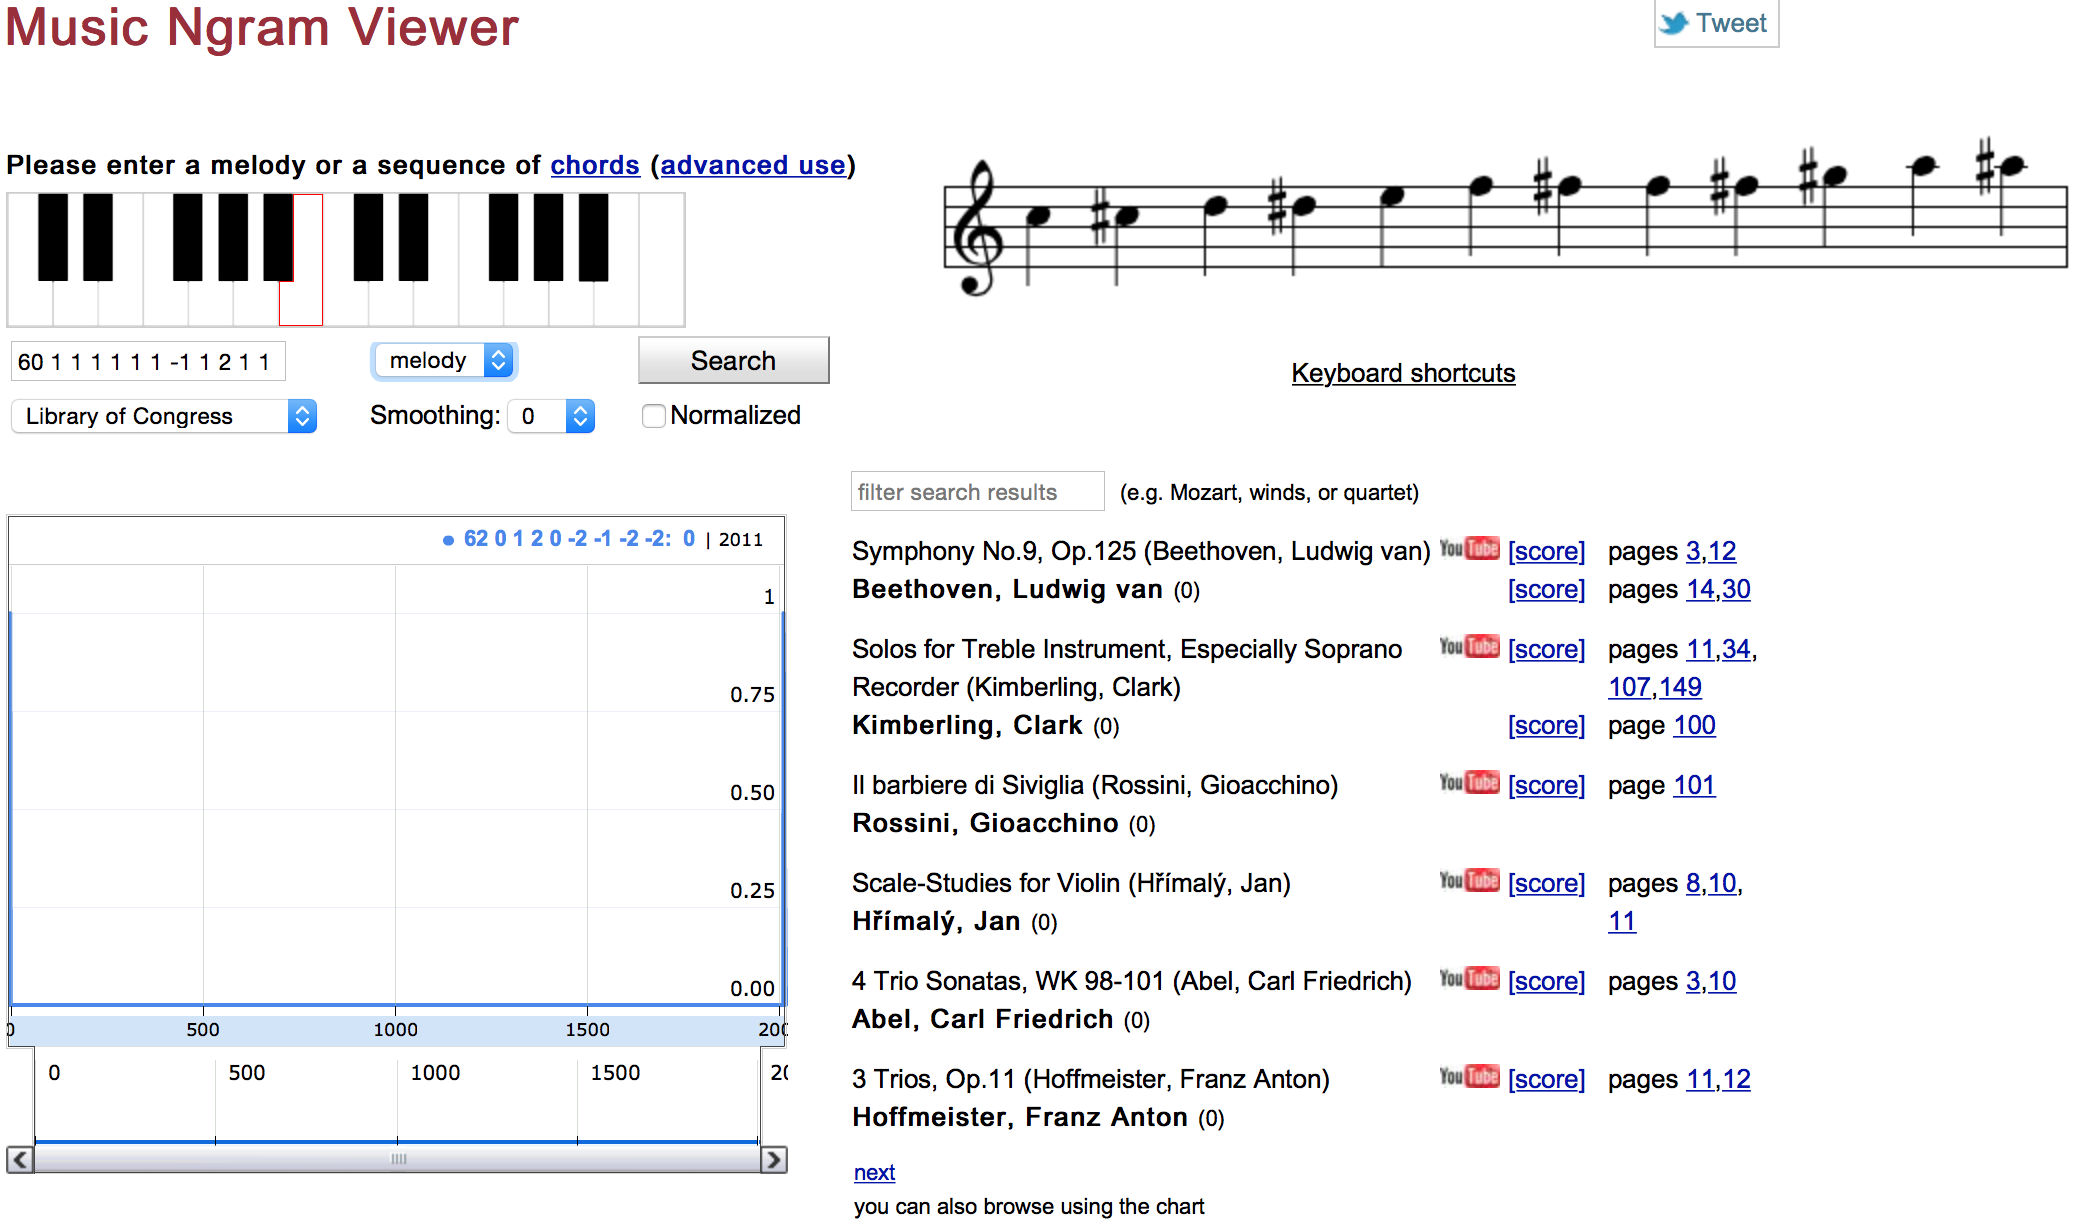
\includegraphics[width=\textwidth]{peachnote}
\caption{Peachnote Ngram Viewer}
\label{fig:peachnote}	
\end{figure}
\floatstyle{plain}
\restylefloat{figure}

Using something similar to the Peachnote interface would make the application more musician-friendly, and would mean that novice musicians would not need to know all of the symbol names in order to query the database.


\subsubsection{Advanced rendering and sound output options}
It is hoped that the project may be expanded so that users can pick and choose what parts and notation are rendered and outputted to sound. 

This would enable the system to be used as a teaching tool, whereby teachers and students could choose to simplify the music by displaying only the symbols they have learned. It would also allow the sound output generator to be used to create accompaniment parts for practice purposes.

\subsubsection{Implementation of paid or subscription APIs}
A further extension of the online API implementation which would be useful is the implementation of new sources which are not open or free. 

This would be useful as these sources, such as MusicNotes which implements a pay-per-piece business model, generally contain a larger variety of sheet music, and at a higher quality as they are generally published by the original arranger or composer.

\subsubsection{Centralisation of APIs}
The current project does all processing of online APIs locally. This could be improved by using a centralised API server, which would communicate with other APIs to access information and scan new files for meta data, which would be stored in a database.

The project would then connect to this API alone, sending formatted query input from the application and receiving suggestions and downloads from the APIs.

This would mean the local user's machine would not have to process XML files which may or may not be requested by the user, and that inclusion of new APIs in the eco system would not require users to update. 

\subsubsection{Online Sharing}
The metadata system currently stores all data to a single SQLite database. This could be expanded in future to offer users the opportunity to upload that data to a centralised online database, in a similar way to the suggested improvement in section 5.3.5.

Users would then be able to browse a larger collection of music from a centralised online point, and request downloads from user created collections. Users who shared their collections would be able to view, accept and reject requests, with an accept resulting in the application uploading the file to the server, sending it to the user requesting the file, and finally, delete the copy on the server.

This functionality would allow users to send files to each other in a more intuitive way than using email or other cloud based services, and wouldn't require much more code or changes to the current system architecture. This may, however, incur problems with licensing which would need to be addressed.
